\chapter{Engineering inequalities and intuition, from equalities}

This section will demonstrate how inequalities

I will derive a simple aircraft problem that will serve as
a demonstration of the intuitive structure of geometric programs, and show
how the feasibility space of the design evolves as we introduce new constraints.

\section{Making feasibility sets explicit}

Consider the simple design problem below, where we define a simple bilinear
monomial equality with respect to x and y, and constrain the sum of the variables
to be less than 2:

\begin{equation*}
\begin{aligned}
& {\text{minimize}}
& & x \\
& \text{subject to}
& & x + y \leq 2,
    & & & xy = \frac{1}{2} \label{simple_moneq}
\end{aligned}
\end{equation*}

We can draw the feasibility set of the above problem in both linear and log space,
as shown in Figure~\ref{f:feas_moneq}. One expects that, given only two variables
and a monomial equality constraint, the feasibility space is
a finite line segment in log-space, and a finite exponential function in linear space.

\begin{figure}
    \centering
    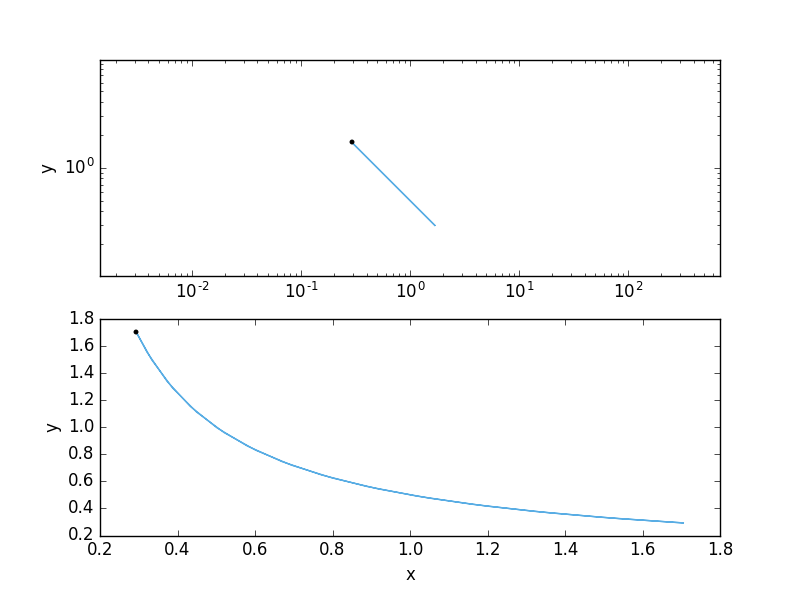
\includegraphics[width=0.8\textwidth]{feas_moneq.png}
    \caption{The x vs y feasibility set of a simple monomial equality.}
    \label{f:feas_moneq}
\end{figure}

However, if we had decided to impose $xy \geq \frac{1}{2}$ instead of \ref{simple_moneq},
then we would get a new feasibility set as shown in Figure~\ref{f:feas_posygeq}.

\begin{figure}
    \centering
    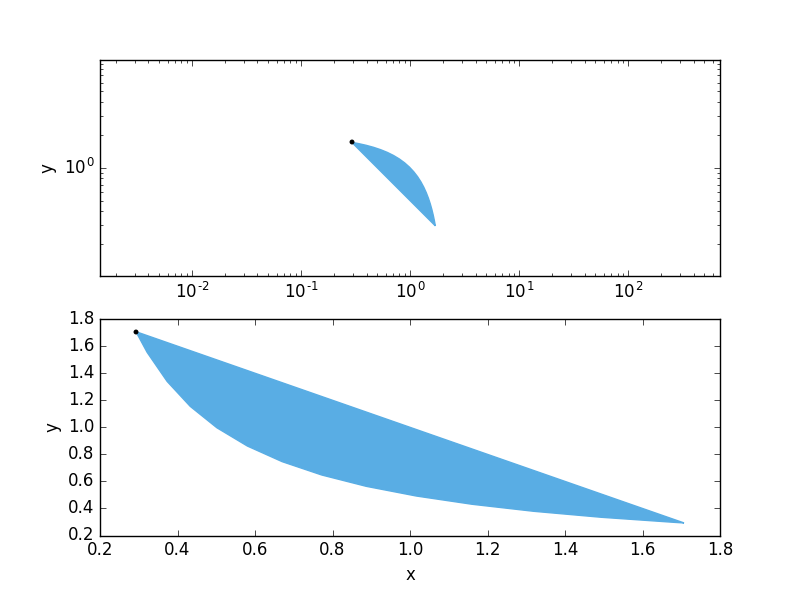
\includegraphics[width=0.8\textwidth]{feas_posygeq.png}
    \caption{The x vs y feasibility set of lower bounding monomial,
    and upper-bonding posynomial.}
    \label{f:feas_posygeq}
\end{figure}

Since we can always upper-bound posynomials, and lower bound both posynomials
and monomials, we cna

%TODO: figure out how to tie this into SimPleAC model building

Note that the optimal point, which is at $x = 1 - \frac{1}{\sqrt{2}}$, $y = 1 + \frac{1}{\sqrt{2}}$,
does not change by the relaxation of the monomial equality. This is a key
observation that allows us to turn most equalities into \gls{GP}-compatible
posynomial inequalities.

\section{Defining the aircraft design problem}

Aircraft epitomize the nature of complex engineering problems. The physical 
relations describing their motion are nonlinear, and all of their subsystems are 
coupled through the primary forces in flight (thrust, weight, lift, drag). 

\subsection{Objective functions}

Objective functions are the way that a designer puts pressure on the variables 
in the constraints. The goal of the aircraft in question will be to carry a given payload
over a distance while minimizing an objective function. To begin with, we will consider
total fuel weight $W_f$ as our objective, which will put
downward pressure on all of the variables that would cause in greater fuel burn, namely
drag and weight.

In many design problems
formulated as \gls{GP}s, many different objectives will put pressure on design
in the same direction. For example, an aircraft designed for fuel weight will look
different than one
that has been designed for total weight or payload-fuel consumption, but all of
these different objective will put a downward pressure on drag and weight.
As such, this model will be able to take in a number of objective functions
and be properly constrained and bounded.

\subsection{Functional description: constraining the problem}

The typical process for designing anything usually involves doing either a
component decomposition or a functional decomposition of the problem. In
this case, we will think about the functional decomposition to create a
basic list of constraints that our aircraft will need to fulfill to be
able to capture the tradeoffs in an aircraft design problem. (In
Section~\ref{s:submodels}, we will examine how thinking about the component decomposition
can help structure large problems.)

What does an aircraft need to be able to do to deliver payload of a distance?
\begin{itemize}
	\item It will need to be able to sustain steady
    level flight with itself and the payload.
    \item It will need to overcome drag.
	\item It will need to contain enough fuel to complete its mission.
	\item The wing will need to be able to sustain the loads it is
    subjected to.
\end{itemize}

Note that these are in now way presented in order of importance, which is part of
the beauty of \gls{GP}. In the basic example, I will choose not to model engines,
and leave this as an exercise
to complete in Section~\ref{s:engine} to improve the model.

\subsection{Beginning to model: weight and lift}

Oftentimes, GP model creation starts haphazardly, with the designer having a
vague idea about the kind of physics that governs a problem, and some basic
set of assumptions about the configuration. In this initial section, we will
generate variables and constraints with abandon, and think about how to make
sure each variable is adequately constrained later.

For this particular design problem, we start by modeling
weight and lift, since the fundamental function of the aircraft is to stay aloft.
The aircraft has weight, which consists of the payload, wing, and fuel weights. 

\begin{equation}
    W \geq W_p + W_w + W_f
\end{equation}

Note that we have already had to make determination about the relations between
the two sides of the equation. Since heavier aircraft burn more fuel, we are justified
to put total weight as greater than the sum of the component weights. Weight relations
are especially amenable to being represented by posynomials, since most objective
functions penalize higher weight.

We would like the aircraft to be able to sustain steady level flight, which means 
that it needs to generate enough lift to carry itself. We use the naive $W \leq L$ 
model below for steady state flight:

\begin{equation}
    W_p + W_w + 0.5 W_f \leq \frac{1}{2} \rho S C_L V^2
\end{equation}

where the lift of the aircraft is equal to weight of the aircraft with half-fuel, 
which is a crude estimate of the average weight of the aircraft throughout the flight.
Again, the \gls{GP} form is seamless here, since lift is related to fuel weight through
induced drag, and so it is pressured downward by the objective function.

We would also like the fully-fueled aircraft to be able to fly at a minimum speed 
of $V_{min}$ without stalling, so we add the following constraint:

\begin{equation}
    W \leq \frac{1}{2} \rho V_{min}^2 S C_{L_{max}}
\end{equation}

Note that, although we could use a monomial equality here, we don't, because this
relation does not need to be tight. It is possible that the aircraft is able to
fly at a velocity slower than $V_{min}$ for a given objective function.

At this point, we have introduced a large set of variables, some of which are input
parameters, and the others free variables. This decision is often the first decision
that and can shape the whole model development process.

The decision of whether to keep variables fixed or variable can be determined by many
factors. In this case, we set the lift coefficient and takeoff speed to be constants since
(1) we would need
more detailed modeling to determine their values. Payload weight is also set
because (2) it would always be unbounded towards zero due to the downward pressure from
the objective. A designer may also fix variables (3) if he/she knows their values with
certainty (eg. gravitational acceleration $g$) or (4) the variable is a normalizing
coefficient (which we will see in Section~\ref{s:datafit}). We will set the values
to those defined in Table~\ref{tab:vars_WandL}.

\begin{footnotesize}
\begin{table}
    \centering
    \begin{tabular}{ l c l c c}
        \toprule
        Variable & Units & Description & Free & Value \\
        \midrule
        $C_L$ & $~\mathrm{-}$ & wing lift coefficient & Y & - \\
        $S$ & $~\mathrm{m^{2}}$ & total wing area & Y & - \\
        $V$ & $~\mathrm{\tfrac{m}{s}}$ & cruising speed & Y & - \\
        $V_{min}$ & $~\mathrm{\tfrac{m}{s}}$ & takeoff speed & N & 25 \\
        $W$ & $~\mathrm{N}$ & total aircraft weight & Y & -\\
        $W_f$ & $~\mathrm{N}$ & fuel weight & Y & -\\
        $W_w$ & $~\mathrm{N}$ & wing weight & Y & - \\
        $W_p$ & $~\mathrm{N}$ & payload weight & N & 6250\\
        \bottomrule
    \end{tabular}
    \label{tab:vars_WandL}
    \caption{Variables introduced in weight vs. lift model. Free variables,
    and constants and their values have been labeled.}
\end{table} \end{footnotesize}

\subsection{Adding additional performance metrics}

As multi-objective designers, we may also be interested in knowing about
additional performance metrics that can serve as part of objective functions. A
few that are particularly relevant to aircraft will be introduced here.

The time of flight of the aircraft, which is a useful metric to calculate cost, is simply the range over velocity:

\begin{equation}
    T_{flight} \geq \frac{\mathrm{Range}}{V}
\end{equation}

The lift-to-drag ratio is also defined: 

\begin{equation}
    L/D = \frac{C_L}{C_D}    
\end{equation}

The new variables we have introduced are detailed in Table~\ref{tab:vars_perfMetrics}.

\begin{footnotesize}
\begin{table}
    \centering
    \begin{tabular}{ l c l c c }
        \toprule
        Variable & Units & Description & Free & Value \\
        \midrule
        $C_D$ & $~\mathrm{-}$ & drag coefficient & Y & - \\
        $C_L$ & $~\mathrm{-}$ & wing lift coefficient & Y & - \\
        $L/D$ & $~\mathrm{-}$ & lift-to-drag ratio & Y & - \\
        $Range$ & $~\mathrm{km}$ & aircraft range & N & 3000 \\
        \bottomrule
    \end{tabular}
    \caption{Variables introduced to define new performance metrics.}
    \label{tab:vars_perfMetrics}
\end{table} \end{footnotesize}

\subsection{More physics: thrust and drag model}

If we attempt to run our current model, we would find that it is unbounded in many variables.
The results are as follows:

\begin{footnotesize}
\begin{table}
    \centering
    \begin{tabular}{ l c l }
        \toprule
        Unbounded variable & Units & Direction \\
        \midrule
        $S$ & $~\mathrm{m^{2}}$ & $\infty$ \\
        $T_{flight}$ & $~\mathrm{hr}$ & $\infty$ \\
        $V$ &  $~\mathrm{\tfrac{m}{s}}$  & $\infty$ \\
        $W_f$ & $~\mathrm{N}$ & $0$ \\
        $W_w$ & $~\mathrm{N}$  & $0$ \\
        \bottomrule
    \end{tabular}
    \label{tab:WandL_unbounded}
    \caption{Unbounded variables in the weight and lift model. More modeling, or direct
    substitutions are required to
    sufficiently bound these variables.}
\end{table} \end{footnotesize}

This is not surprising at all, since none of the defined variables lower bound $W_f$,
the objective function.

For initial modeling purposes, I assume a constant brake
specific fuel consumption (BSFC) for the 'engine' of the aircraft, which is assumed
to provide as much thrust as needed. Since $T \geq D$:

\begin{equation}
    W_f \geq BSFC \times T_{flight} \times D
\end{equation}

the fuel weight required is the product of the BSFC, time of flight, and the total drag on the aircraft.
The drag of the aircraft is the product of dynamic pressure ($\frac{1}{2} \rho V^2$),
the planform area $S$, and the coefficient of drag of the aircraft:

\begin{equation} 
    D \geq \frac{1}{2} \rho V^2 S  C_D
\label{e:d}
\end{equation}

There is yet another relaxed monomial equality in Equation~\ref{e:d}.
If the pressure on the \gls{LHS} or \gls{RHS} of a monomial equality are clear as in this case,
it is a good practice to relax the equality to leave as many degrees of freedom
in the design space as possible.

The drag coefficient of the aircraft is assumed to be the sum of the fuselage drag,
the wing profile drag, and the wing induced drag coefficients:

\begin{equation}
    C_D \geq C_{D_{fuse}} + C_{D_{wpar}} + C_{D_{ind}}
\label{e:cd}
\end{equation}

The fuselage drag is a function of its drag area $CDA_0$ and the planform area of the wing:

\begin{equation}
    C_{D_{fuse}} = \frac{CDA_0}{S}
\label{e:cdfuse}
\end{equation}

where the $CDA_0$ is linearly proportional to the volume of fuel in the fuselage:

\begin{equation}
    V_{f_{fuse}} \leq CDA_0 \times 10 ~\mathrm{[meters]}
\label{e:vffuse}
\end{equation}

Note that we correct the dimensionality of the volume here, since GPkit automatically checks units. 

The wing profile drag is the product of the form factor, the friction drag coefficient,
and the wetted area ratio of the wing,

\begin{equation}
    C_{D_{wpar}} = k C_f S_{wetratio}
\label{e:cdwpar}
\end{equation}

The Reynolds number of the aircraft wing is approximated

\begin{equation}
    Re \leq \frac{\rho}{\mu} V \sqrt{\frac{S}{AR}}
\label{e:re}
\end{equation}

and used to find the friction drag coefficient of wing. We approximate the $C_f$ by assuming a turbulent Blasius flow over a flat plate as below:

\begin{equation}
    C_f \geq \frac{0.074} {Re^{0.2}}
\end{equation}

The induced drag of the wing is calculated with a span efficiency factor e, and is a function of the $C_L$ and aspect ratio $AR$ of the wing.

\begin{equation}
    C_{D_{induced}} = \frac{C_L^2}{\pi AR e}
\label{e:cdinduced}
\end{equation}

\begin{python}
        # Thrust and drag model
        C_D_fuse = CDA0 / S
        C_D_wpar = k * C_f * S_wetratio
        C_D_ind  = C_L ** 2 / (np.pi * A * e)
        constraints += [W_f >= BSFC * T_flight * D,
                    D >= 0.5 * rho * S * C_D * V ** 2,
                    C_D >= C_D_fuse + C_D_wpar + C_D_ind,
                    V_f_fuse <= 10*units('m')*CDA0,
                    Re <= (rho / mu) * V * (S / A) ** 0.5,
                    C_f >= 0.074 / Re ** 0.2]
\end{python}

\subsection{Boundedness as a GP}

\begin{footnotesize}
\begin{table}
\begin{tabular}{ l c l }
    \toprule
	Unbounded variable & Units & Direction \\
    \midrule
    $V_{f_{fuse}}$ &  $~\mathrm{m^3}$  & $0$ \\
    $W_w$ & $~\mathrm{N}$  & $0$ \\
    \bottomrule
\label{tab:WLTD_unbounded}
\end{tabular}
\end{table} \end{footnotesize}

As shown in Table~\ref{tab:WLTD_unbounded} attempting to run the model as is
results in both the fuselage fuel
volume $V_{f_{fuse}}$ and the wing weight $W_w$ being lower-unbounded. Next,
I will attempt to properly bound these to complete the SimPleAC model.

\section{Limits of GP and Convexity} \label{s:GPLimits}

Even with the demonstrated strengths of \gls{GP}'s in solving certain classes of 
problems, it is important to recognize that the mathematical framework has limits. 
Certain constraints can only be expressed as signomial constraints, which are 
non-log-convex extensions of posynomial constraints. Even the addition of a single 
signomial constraint turns the problem from a \gls{GP} to a \gls{SP}, which means
that the problems loses convexity and all of the mathematical guarantees associated with it. 
It takes engineering intuition to recognize where and when improved modeling is worth
the loss of the mathematical guarantees.

\subsection{Introducing fuel volume constraints to a GP aircraft model}

To demonstrate a model that requires the addition of signomial constraints, we will 
be adding a fuel volume model to SimPleAC, where fuel can be stored in the wing or
in the fuselage. The reason why this model is GP-incompatible is because of the 
following constraint which follows logically:

\begin{equation}
	V_{f_{avail}} \leq V_{f_{wing}} + V_{f_{fuse}}
	\label{vfavail}
\end{equation}

The fuel volume available must be less than the sum of the fuel volume available in the
wing and the fuselage. As such, it turns out that volumes that 'contain' free variables
can create signomial constraints. (One way around this is potentially creating fuel
fraction variables to denote how much fuel is stored in each volume, but I will not 
explore other potential parametrizations here.)

As such, we can continue to develop the model. We know that fuel weight is going 
to influence the lift required of the aircraft, so we must determine the weight of the fuel 
using a density parameter $\rho_{f}$. 

\begin{equation}
    V_f = \frac{W_f } {\rho_f g}
    \label{e:vf}
\end{equation}

We need a model of how much fuel volume there is in a wing. If we think about the total
volume in a wing, it is related linearly to its thickness ratio ($\tau$) and span ($b$), 
and to the square of its chord ($c$). 

\begin{equation}
	V_{f_{wing}} \propto \tau b c^2
	\label{e:vfwingpre}
\end{equation} 

In aerospace engineering, we like dimensionless quantities and planform areas, 
so we would like to express relation~\ref{e:vfwingpre} with respect to the planform area $S$
aspect ratio \AR and thickness ratio $\tau$ only, without having to define $b$ and $c$ as new
free variables.
Using the additional relation $S \propto b c$, we can express $V_{f_{wing}}$.

\begin{equation}
	V_{f_{wing}} \propto \tau (\frac{AR}{S})^{0.5} (\frac{S}{b})^2 \propto
		(\frac{AR}{S})^{0.5} \frac{S^2}{S \AR} \propto \frac{\sqrt{S}\tau}{\sqrt{AR}}
\end{equation}

\begin{equation}
\label{e:vfwing}
V_{f_{wing}}^2 \leq 9\times10^{-4} \frac{S \tau^2}{AR}
\end{equation}

(In the final form of the Equation~\ref{e:vfwing} I picked $9\times10^{-4}$ as the coefficient in
front of the relation by tuning it after I had developed
the model, but any other coefficient would do.)

\subsection{What is the proper use case of the signomial equality?} 

Signomial equalities must be used as a last resort. The signomial equality is the only place 
where the feasibility set of individual \gls{GP}'s within a \gls{SP} solve are not guaranteed 
to be subsets of the feasibility set of the \gls{SP}. This is undesirable although
the solution of the \gls{SP} with equalities is guaranteed to be in the feasibility region
of the model.
